% Template for PLoS
% Version 3.1 February 2015
%
% To compile to pdf, run:
% latex plos.template
% bibtex plos.template
% latex plos.template
% latex plos.template
% dvipdf plos.template
%
% % % % % % % % % % % % % % % % % % % % % %
%
% -- IMPORTANT NOTE
%
% This template contains comments intended 
% to minimize problems and delays during our production 
% process. Please follow the template instructions
% whenever possible.
%
% % % % % % % % % % % % % % % % % % % % % % % 
%
% Once your paper is accepted for publication, 
% PLEASE REMOVE ALL TRACKED CHANGES in this file and leave only
% the final text of your manuscript.
%
% There are no restrictions on package use within the LaTeX files except that 
% no packages listed in the template may be deleted.
%
% Please do not include colors or graphics in the text.
%
% Please do not create a heading level below \subsection. For 3rd level headings, use \paragraph{}.
%
% % % % % % % % % % % % % % % % % % % % % % %
%
% -- FIGURES AND TABLES
%
% Please include tables/figure captions directly after the paragraph where they are first cited in the text.
%
% DO NOT INCLUDE GRAPHICS IN YOUR MANUSCRIPT
% - Figures should be uploaded separately from your manuscript file. 
% - Figures generated using LaTeX should be extracted and removed from the PDF before submission. 
% - Figures containing multiple panels/subfigures must be combined into one image file before submission.
% For figure citations, please use "Fig." instead of "Figure".
% See http://www.plosone.org/static/figureGuidelines for PLOS figure guidelines.
%
% Tables should be cell-based and may not contain:
% - tabs/spacing/line breaks within cells to alter layout or alignment
% - vertically-merged cells (no tabular environments within tabular environments, do not use \multirow)
% - colors, shading, or graphic objects
% See http://www.plosone.org/static/figureGuidelines#tables for table guidelines.
%
% For tables that exceed the width of the text column, use the adjustwidth environment as illustrated in the example table in text below.
%
% % % % % % % % % % % % % % % % % % % % % % % %
%
% -- EQUATIONS, MATH SYMBOLS, SUBSCRIPTS, AND SUPERSCRIPTS
%
% IMPORTANT
% Below are a few tips to help format your equations and other special characters according to our specifications. For more tips to help reduce the possibility of formatting errors during conversion, please see our LaTeX guidelines at http://www.plosone.org/static/latexGuidelines
%
% Please be sure to include all portions of an equation in the math environment.
%
% Do not include text that is not math in the math environment. For example, CO2 will be CO\textsubscript{2}.
%
% Please add line breaks to long display equations when possible in order to fit size of the column. 
%
% For inline equations, please do not include punctuation (commas, etc) within the math environment unless this is part of the equation.
%
% % % % % % % % % % % % % % % % % % % % % % % % 
%
% Please contact latex@plos.org with any questions.
%
% % % % % % % % % % % % % % % % % % % % % % % %

\documentclass[10pt,letterpaper]{article}
\usepackage[top=0.85in,left=2.75in,footskip=0.75in]{geometry}

% TODO remove before submission
\usepackage{mathptmx}

% Use adjustwidth environment to exceed column width (see example table in text)
\usepackage{changepage}

% Use Unicode characters when possible
\usepackage[utf8]{inputenc}

% textcomp package and marvosym package for additional characters
\usepackage{textcomp,marvosym}

% fixltx2e package for \textsubscript
\usepackage{fixltx2e}

% amsmath and amssymb packages, useful for mathematical formulas and symbols
\usepackage{amsmath,amssymb}

\DeclareMathOperator*{\argmin}{arg\,min}

\DeclareMathOperator*{\argmax}{arg\,max}

% cite package, to clean up citations in the main text. Do not remove.
\usepackage{cite}

% Use nameref to cite supporting information files (see Supporting Information section for more info)
\usepackage{nameref,hyperref}

% line numbers
\usepackage[right]{lineno}

% ligatures disabled
\usepackage{microtype}
\DisableLigatures[f]{encoding = *, family = * }

% rotating package for sideways tables
\usepackage{rotating}

% Remove comment for double spacing
%\usepackage{setspace} 
%\doublespacing

% Text layout
\raggedright
\setlength{\parindent}{0.5cm}
\textwidth 5.25in 
\textheight 8.75in

% Bold the 'Figure #' in the caption and separate it from the title/caption with a period
% Captions will be left justified
\usepackage[aboveskip=1pt,labelfont=bf,labelsep=period,justification=raggedright,singlelinecheck=off]{caption}

% Use the PLoS provided BiBTeX style
\bibliographystyle{plos2015}

% Remove brackets from numbering in List of References
\makeatletter
\renewcommand{\@biblabel}[1]{\quad#1.}
\makeatother

% Leave date blank
\date{}

% Header and Footer with logo
\usepackage{lastpage,fancyhdr,graphicx}
\usepackage{epstopdf}
\pagestyle{myheadings}
\pagestyle{fancy}
\fancyhf{}
\lhead{\includegraphics[width=2.0in]{PLOS-submission.eps}}
\rfoot{\thepage/\pageref{LastPage}}
\renewcommand{\footrule}{\hrule height 2pt \vspace{2mm}}
\fancyheadoffset[L]{2.25in}
\fancyfootoffset[L]{2.25in}
\lfoot{\sf PLOS}

\usepackage{subcaption}

%% Include all macros below

\newcommand{\lorem}{{\bf LOREM}}
\newcommand{\ipsum}{{\bf IPSUM}}

%%%%%%%%%%%%%%%%%%%%%%%%%% REMOVE BEFORE SUBMISSION %%%%%%%%%%%%%%%%%%
\usepackage[colorinlistoftodos]{todonotes}
\setlength{\marginparwidth}{2cm}
\reversemarginpar




%% END MACROS SECTION


\begin{document}
\vspace*{0.35in}

% Title must be 250 characters or less.
% Please capitalize all terms in the title except conjunctions, prepositions, and articles.
\begin{flushleft}
%{\Large
%\textbf\newline{Can We Identify Transmission Bias in the Archaeological Record?  An Investigation of Equifinality Using Classifier Methods}
%}
{\Large
\textbf\newline{We Cannot Easily Identify Biased Cultural Transmission in the Archaeological Record}
}
\newline
% Insert author names, affiliations and corresponding author email (do not include titles, positions, or degrees).
\\
Mark E. Madsen\textsuperscript{1,*}


\bf{1} Department of Anthropology, Box 353100, University of Washington, Seattle, WA 98195-3100, USA
\\
\bigskip

% Insert additional author notes using the symbols described below. Insert symbol callouts after author names as necessary.
% 
% Remove or comment out the author notes below if they aren't used.



% Use the asterisk to denote corresponding authorship and provide email address in note below.
* mark@madsenlab.org

\end{flushleft}
% Please keep the abstract below 300 words
\section*{Abstract}
Lorem ipsum dolor sit amet, consectetur adipiscing elit. Curabitur eget porta erat. Morbi consectetur est vel gravida pretium. Suspendisse ut dui eu ante cursus gravida non sed sem. Nullam sapien tellus, commodo id velit id, eleifend volutpat quam. Phasellus mauris velit, dapibus finibus elementum vel, pulvinar non tellus. Nunc pellentesque pretium diam, quis maximus dolor faucibus id. Nunc convallis sodales ante, ut ullamcorper est egestas vitae. Nam sit amet enim ultrices, ultrices elit pulvinar, volutpat risus.


\linenumbers

\section{Introduction}\label{introduction}

The emerging field of \emph{cultural evolution} is the study of cultural change in humans and other animals as a Darwinian evolutionary process, and encompasses research in biology and the social sciences \cite{dunnell1980evolutionary,laland2011sense,8893,Mesoudi:2007,Mesoudi2015Cultural-Evolut,o2000applying}.\footnote{Cultural evolution, in the sense used here, is distinct from the Spencerian version common in the social sciences from the late 1800's through the present, which is progressive and unilinear \cite{morgan1877ancient,tylor1874primitive,white1949science}.  Since vestiges of progressivist cultural evolution are still common enough in anthropology and archaeology, the choice of the term to describe a contemporary, and thoroughly Darwinian, field of research is unfortunate, but it appears to be taking root among practitioners and so I employ it here.}  Drawing upon the formal principles of Darwinian evolutionary biology (best articulated by Lewontin \cite{Lewontin1970}) and now-classic quantitative frameworks by Cavalli-Sforza and Feldman \cite{CF1981} and Boyd and Richerson \cite{BR1985}, cultural evolution combines population thinking with an understanding of the differences between genetic and cultural transmission.  Chief among these differences is the importance of cognitive or psychological biases which shape how social learning of skills and cultural traits occurs.  Over the past twenty years, experiments, observational studies, and theoretical models have come together to give us a picture of human social learning which is conformist and payoff-biased (for an introduction to a very large literature on this point, see \cite{boyd2005origin,Henrich:2001p5229,8897,laland2004social,8895,Mesoudi2015Cultural-Evolut}).  

Most of the evidence for our emerging picture of human social learning comes from controlled experiments and observational studies of living populations performed by psychologists and anthropologists \cite{henrich2011fiji}\todo{REFS}.  Such experiments give us insight into the mechanisms of social learning favored within human populations, among many possible learning mechanisms.  Using this knowledge in empirical research, though, requires that we understand the performance of theoretical models of social learning in the \emph{model selection} task.  In model selection, we attempt to infer or estimate the model among a set of models which best fits our data.  Moreover, in most empirical situations, we will not be performing model selection with fine grained, individual level data, but instead with coarse grained, population level data.  In this paper, I consider coarse grained data to be composed of the frequencies of cultural variants measured within a population or some archaeological unit which represent artifacts from a population or populations.  

Understanding the limitations of using coarse grained data to perform model selection among social learning models is crucial for archaeology and paleoanthropology in particular, since both disciplines inherently rely upon sampling a sedimentary record of artifact discard across the landscape.  Except in the very rarest of cases, archaeological samples reflect the activities of many individuals, and thus are inherently coarse-grained \cite{Shennan2011}.  Archaeologists employing cultural transmsision models in their research have a long-standing research interest in solving this model selection problem.  The main approach has been to identify summary statistics from population-level frequency data that seem to be diagnostic of particular social learning models.  In particular, much of the focus in this literature has been differentiation of cognitive biases such as conformism, anti-conformism, or pro-novelty biases \cite{Bentley2003,bentley2004random,bentley2007regular,Blythe2011space,Crema:2014ef,Evans:2011vm,kandler2013non,kohler2004,Mesoudi2009,Rorabaugh:2014fl,steele2010ceramic}.   Examples of statistical properties which may reveal the population-level consequences of different evolutionary models include various measures of the richness or diversity (evenness) of traits, the average amount of time that traits survive in the population, the exponent in a power-law distribution of variant frequencies, or the degree to which frequency data match distributions known to arise in appropriate null models \cite{Mesoudi2009}.  These variables are highly attractive for archaeological purposes because most of them are easy to calculate from standard descriptions of archaeological assemblages.  

The initial optimism stemming from success in separating social learning models given ideal simulated samples is giving way more recently to skepticism, however, as models begin to incorporate more realism in representing sampling and the processes inherent in formation of the archaeological and fossil records \cite{Kandler20150905,Madsen2012TA,wilderkandler2015}.  Archaeological deposits are time-transgressive accumulations of artifacts deposited over time, and even fine grained recovery techniques will typically yield samples which are time averaged and small in comparison to the total population of artifacts discarded by past peoples.   Given work by Premo, Porčić, and myself, we now understand that when the artifact assemblages which form our counting units accumulate over period of time which is large compared to the rate at which variants change in the population, some statistical tests may lack power and suffer high error rates in identifying the correct social learning process \cite{Madsen2012TA,Porcic2014Exploring-the-E,Premo:2014jv}.  Kandler and colleagues have shown, in parallel, that sparse and small samples markedly hamper our ability to differential social learning models from summary statistics in coarse grained data, 


Other research has shown the effect of non-stationary population size on inferring transmission bias \cite{Rorabaugh:2014fl}, and Kandler and colleagues have convincingly demonstrated that inference is strengthened using diachronic statistics from nonequilibrium models of cultural transmission models \cite{kandler2013non, wilderkandler2015}.  They \cite{wilderkandler2015} additionally call out the role of sample size, noting that sparse and small samples markedly hamper the ability to statistically identify social learning models.  

Initial optimism about finding robust methods for selecting among social learning models is giving way to skepticism given more realism in our theoretical studies , and rightly so.  Social learning models are fundamentally stochastic diffusion processes, and the sparser and more aggregated our observations of such processes are, the greater the degree to which different models or parameterizations of a model will display equifinality.  The practical question is whether equifinality is widespread, or relatively rare?  If relatively rare, then model selection among different social learning modes from archaeological contexts is a potentially useful research strategy.  If equifinality is the rule with realistic assemblage conditions (e.g., time averaging and sample size), then we would be well advised to seek coarser grained research questions to match our coarse grained data.  This question is depicte schematically in Fig. \ref{fig1}.  In the left panel, under mild to moderate amounts of time averaging and with most reasonable sample sizes, our ability to identify transmission bias is strong, and problems identifying bias are restricted to situations with small sample sizes and significant temporal aggregation.  The right hand panel depicts the opposite situation where identification of transmission bias is rare across a range of values, and may only be possible with relatively complete samples and without significant time averaging.  

\todo{stopped editing here}





In order to answer this, we need to know several things.  First, which statistical properties give the best discriminatory power, either singly or when employed in combination?  Second, how do sampling and time averaging combined (not separately) affect identification?  In this paper, I approach these issues by examining a large sample of simulated conformist, anticonformist, and unbiased transmission events through ``data collection regimes'' comprised of different sample fractions and durations of temporal aggregation.  For each model and data collection regime, I measured a set of diversity, distributional, and diachronic statistics.  The result is a large compendium of measured statistics across data collection regimes which approximate sparse to complete samples of the archaeological record, over spans of temporal aggregation which approximate short almost synchronic intervals, to periods of accumulation very long compared to the behavioral time scale.  

\begin{figure}[h]
\caption{How rare are the circumstances under which we have a strong ability to identify transmission bias in archaeological samples?  Two possible outcomes are shown.  In the left panel (A), difficulty in separating transmission models are restricted to situations where sample fractions are very small and time averaging is very large, leaving a region where our ability to distinguish models is strong for short-duration assemblages.  In the right panel (B), it is difficult to identify distinguish transmission bias from an unbiased model given most sampling regimes and with any significant time averaging.}
\label{fig1}
\end{figure}


Given this type of data set compendium of measured statistics, we can begin to map where identification of transmission bias is possible and where our ability to discern bias breaks down.  I measure the ability to detect transmission bias as the ability to correctly classify samples as to their model of origin \cite{devijver1982pattern, fukunaga1990introduction, hastie2009elements}, while equifinality between models is indicated by poor classification performance and high error.\footnote{Throughout this paper, I used ``classification'' in the statistical and machine-learning sense of a statistical model whose dependent variable is a binary or discrete value, such that the model predicts which value a data point takes from a labeled set.  Archaeologists will be accustomed to using the term in the sense of systematics and taxonomy, which is not the intent here.}  Since we want to find the minimum possible classification error, I employ gradient boosted classification trees, for their superb performance on many classification tasks, ability to automatically capture interactions between variables, and ability to indicate the relative importance of variables to classification performance \cite{AlexeyNatekin:2013ew,hastie2009elements}. 

The results indicate that while neutral and biased transmission models
can be distinguished very accurately given measurements from entire
populations taken when no temporal aggregation occurs, the introduction of
sampling and the interaction between sampling and time averaging markedly degrades our ability to distinguish these transmission
rules. Furthermore, the degradation is not symmetric. With sampled, time
averaged data, we are extremely likely to conclude that samples
represent biased transmission, even when this is not the case.  This result has potential implications for interpreting the results of past studies, and it certainly calls into question whether archaeologists can fruitfully engage in the kind of ``microevolutionary'' analysis implied by the identification of cognitive social learning biases.  I conclude with a discussion of coarse-grained questions and methods which may better leverage the unique strengths of a diachronic, time averaged archaeological record.




\section{Materials and Methods}
\label{analysis}


\subsection{Identifying Transmission Bias Using Statistical Classifiers}
\label{sec:equifinality-classification-error}

The ability to identify transmission bias in archaeological samples of class or type frequencies is dependent upon finding values of statistical measures, or functional forms for frequency distributions, which are distinctive among a set of models (for example, between conformist and unbiased transmission).  Previous studies employ both approaches.  Kohler and colleagues \cite{kohler2004} built on Neiman's pioneering work \cite{Neiman:1995p23690}, and compare the expected amount of design diversity (technically, richness) one would expect to see in assemblages given either conformist or unbiased transmission (finding evidence for the former at Burnt Mesa Pueblo in New Mexico).  On the distributional front, in a series of papers Bentley has stressed the functional form or slope of the class frequency distribution, claiming that departures from a power law distribution are indicative of transmission bias \cite{Bentley2003,bentley2004random,bentley2007regular}, which was supported and extended in simulations by Mesoudi and Lycett \cite{Mesoudi2009}.  

These approaches to identification are similar in looking for a single, low-dimensional discriminator, and while it is useful to find the simplest possible means of discriminating between models, the existence and nature of a simple discriminator does not answer the question of whether transmission models can be distinguished from frequency data, or whether significant equifinality exists.  For the latter, we need to understand the degree to which the behavior of our social learning models overlaps not just along a single dimension, but in the full space of all variables we can measure.  To see why, consider an artificial example in which two variables are measured on the outcomes of two cultural transmission models (Fig. \ref{fig2}), with one model shown in dark grey, and the other in light blue.  In the left hand panel (A), it is clear that neither predictor variable cleanly separates the two models on their own, but that a linear combination of the two predictors provides near-perfect identification of each transmission model based upon just two measurements (in this hypothetical example, perhaps one predictor is Neiman's $t_f$ diversity measure, and the other is Slatkin's ``exact'' test for conformance to the Ewens Sampling Formula \cite{Neiman:1995p23690,slatkin1994exact}).  In contrast, the middle panel (B) presents a much harder challenge, with most of the distributions overlapping, and only points at the bottom and top extremes of the distributions secure in their model identification.  Finally, in the right panel (C), the overlap is too significant to conclude that we can identify either model given these predictor variables:  the transmission models are equifinal and indistinguishable in this case. 

\begin{figure}[h]
\caption{Simple example of model outcomes with different degrees of distinguishability: (A) simulated data point from two fully separate models, (B) two models with a limited overlap region, (C) and two models whose outcomes are highly overlapping.}
\label{fig2}
\end{figure}

All other things being equal, if we add more predictor variables and view the outcomes of our transmission models as a higher-dimensional data set (which is hard to visualize on the page, but easy to conceive), there should be a better chance of finding a relationship among variables that separates the models, since the data points become scattered through a much larger volume (given the larger dimensionality of the space).   That relationship may not be a simple straight line (or its higher-dimensional analogue, a ``hyperplane'', given many variables), but may involve interactions between variables which are expressed as nonlinear terms.  Finding  relationships among variables which separate classes of observations is the statistical problem of ``classification'' or ``pattern recognition,'' and the problem of determining whether such a relationship exists boils down to finding the optimal classification rule.  If the optimal or best-performing classification rule has high accuracy, then we can securely identify instances of a transmission model given statistical measurements on data consisting of artifact class frequencies.  If, on the other hand, the best possible classification rule we can construct is accurate little more than 50\% of the time, then considerable equifinality exists and we cannot identify transmission bias in our data.  The key is to find or approximate that optimal classification rule.

Given a set of $k$ transmission models \(\mathcal{M}_1 \ldots \mathcal{M}_k\), and a set of $p$ variables or statistics \(s_1 \ldots s_p\) that we can measure on the outcomes of those models (across a set of input parameters, of course), there are usually many possible classification rules for predicting the model which generated a given sample, and those possible rules will vary widely in their quality.  There is guaranteed to be a maximally accurate rule (or rules), however, which has the minimum possible error in separating observations from different models.  This error may not be zero, and will not be in cases such as Fig. \ref{fig2} panels B and C, where model outcomes significantly overlap.  The rule which has the minimum error is the rule whose probability of correct assignment is highest, given the conditional density of the data for each model, across the parameters.  This sounds like an application of Bayes' theorem, and in fact we can write the classification error problem as follows, where
\(Y \in 1, \ldots, K\) refers to each of \(k\) models, and
\(X_1, \ldots, X_p\) refer to \(p\) different predictor variables.

\begin{equation}
\mathbb{P}(Y | X_1, \ldots, X_p) = \frac{\mathbb{P}(Y_i) \mathbb{P}(X_1, \ldots, X_p | Y)}{\mathbb{P}(X_1, \ldots, X_p)}
\label{eq:bayes-rule-classification}
\end{equation}

\(\mathbb{P}(Y)\) plays the role of the prior distribution, and is the
prevalence of each model in the population.\footnote{In this simplified presentation, the actual parameters of each model are not shown, but they would be hyperparameters in the overall analysis.}  Thus, the most probable generating model for a given data point is simply the mode of the likelihood function, given by:

\begin{equation}
Y_{pred} = \argmax_y \mathbb{P}(X_1, \ldots, X_p | Y)
\label{eq:map-class-bayes}
\end{equation}

This is the \emph{Bayes classifier} for a controlled simulation
experiment, and its error rate in separating data points by model is
called the \emph{Bayes error}. This is the lowest possible error in
separating the models given the data
\cite{devijver1982pattern, fukunaga1990introduction, hastie2009elements}.
The Bayes error is zero when we can correctly identify each data point
as to its model of origin (as in the left panel of Fig. \ref{fig1}, and rises as model outcomes overlap in the
measurement space. With sufficient overlap, the Bayes error could
approach $1/k$ for $k$ models, which represents a prediction rule which is no better than
chance.\footnote{Predictors can achieve even worse error levels, performing more poorly than coin-flipping, but in the current study we will not encounter such rates.}

This summarizes the decision theory behind using classifier models to assess our ability to identify transmission bias (or, conversely, to detect equifinality among models).  We almost never have the ability to calculate the Bayes error directly, since we rarely have an explicit (or solvable) expression for the likelihood function in Eq. \ref{eq:bayes-rule-classification} or \ref{eq:map-class-bayes}.  In fact, the Bayes error rate is only calculable in very special cases, such as Gaussian distributions where all models/classes share the same covariance matrix.\footnote{There is a large literature, especially in pattern recognition and language classification, on approximating upper bounds for the Bayes error of a classifier, because it is highly useful to know when you cannot improve a recognition system or classifier any further \cite{Antos:1999dn, Dobbin:2009du, McLachlan:1975eo}.  Most such upper bounds are based upon parametric models, and use estimates of a distance metric between the classes being distinguished (typically, the Mahalanobis or Bhattacharyya distance) \cite{devijver1982pattern}.  Such bounds are difficult to justify in situations where we have complex social learning models, whose probability density functions in the space of measured variables are typically unknown and are unlikely to be Gaussian.  Non parametric bounds are possible, using nearest-neighbor methods \cite{Loizou:1987bi}, but in most cases the values obtained are not very tight and the performance of boosting and bagged classifiers easily surpasses such methods.}  In practice, the Bayes error rate is approximated numerically, using a statistical classifier algorithm which is known to have near optimal performance on the same data types one is analyzing.  The choice of gradient boosted classification trees for this study is described further in Section \ref{classifier-selection-and-training}.  


\subsection{Study Design}
\label{study-design}





\subsection{Cultural Transmission Models}\label{simulated-samples-of-cultural-transmission-models}



\subsection{Observable Variables}
\label{variable-selection}



\subsection{Data Collection Treatments}
\label{data-collection-treatments}


\subsection{Classifier Selection, Training, and Evaluation}
\label{classifier-selection-and-training}

There are several families of classifier algorithms which outperform familiar methods like logistic regression, and are known to be near-optimal on a variety of data sets.  In particular, ensemble algorithms which combine many individual predictions to reduce variance and the effect of outliers achieve some of the best out-of-sample or generalization error in systematic tests \cite{hastie2009elements}, and thus come closest to estimating the
Bayes rate \cite{tumer2003bayes}.  There can be no single ``best'' algorithm.  A very general result in statistical decision theory (called, appropriately, the ``no free lunch'' theorems) show that no single prediction model can achieve the best result across all combinations of data and parameters \cite{wolpert2002supervised, wolpert1997no}.  Thus, algorithms are usually evaluated using an empirical approach, running comparisons across a large number of test data sets.  Fern\'{a}ndez-Delgado \cite{Fernandez-Delgado:2014:WNH:2627435.2697065} compared the performance of 179 classifiers from 17 families of statistical methods across 121 data sets drawn from the UC Irvine repository of machine learning data sets.  Their study found that random forests \cite{breiman2001random}, support vector machines,
and various types of boosted classifiers \cite{hastie2009elements} performed the best.

In selecting a classifier algorithm for this study, I want near optimal accuracy but also a relative sense of which predictor variables are important.  The goal is not merely to be able to detect transmission bias, but also to understand what variables will help us do so.  Support vector machines do not offer an easily understood measure of variable importance given their construction, and thus were not considered in this study.  I generated a small test data set, independent of the simulations used for the main study, and tested the accuracy of R language implementations of both Leo Breiman's original random forest algorithm, and gradient boosted machines.\footnote{The data for this initial comparison are available in the \url{https://github.com/mmadsen/experiment-ctmixtures} repository under the experiment name ``equifinality-2''.}  In that calibration data set, gradient boosted models slightly outperformed random forests, and were superior in computational cost, and are used for all further results in this paper.  

Gradient boosted classification operates by repeatedly fitting a set of
decision trees to the data \cite{AlexeyNatekin:2013ew,hastie2009elements}. In each round, decision trees are fit to the training data, and individual data points scored as errors or successful predictions.  Subsequent trees are fitted by modifying the trees in the direction that minimizes the residual error.  This is equivalent to finding the gradient of the loss function in the space of possible classifier functions, hence the name of the method.  The impact of each gradient step is smoothed by including a ``shrinkage'' factor.  Finally, the gradient steps are ``boosted'' to weight data points by the success in prediction, such that data points that are frequently misclassified become targeted by the algorithm until they can be correctly predicted \cite{freund1995boosting, freund1999short, schapire2012boosting}.  After a specified number of iterations, the class or label membership of each data point is obtained by having each gradient step classifier tree ``vote'' for class membership, and the final answer is the majority vote.  This class of models can also be visualized as repeated refitting of residuals until error is minimized \cite{friedman2001greedy}.  This combination of boosting and iterative function search is very powerful, and accounts for gradient boosted algorithms regularly outperforming many other families of classifiers.

In this study, I employ the R package (\textbf{gbm}) for gradient
boosted classification \cite{ridgeway1999state}, with the binomial deviance \(\textrm{log}(1 + \textrm{exp}(-2y\hat{y}))\) as our loss function, where \(y\) is the true
model for a data point, and \(\hat{y}\) is the classifier model's
prediction.  Binomial deviance approximates the ``zero-one'' loss function with one which is differentiable, which is needed for a gradient descent method.  

For each of the comparisons described in Section \ref{study-design}, a GBM classifier was trained on 80\% of the variable measurements from a set of simulation output.  The remaining 20\% were held back as a test data set to evaluate the accuracy of the classifier on data independent of the training data.  Gradient boosted machines take a number of tuning hyperparameters (number of boosting iterations, depth of classification trees).  Rather than selecting these by convention or using arbitrary values, these parameters were tuned using 5 rounds of repeated 10-fold cross-validation on the training data to select optimal values \cite{Kim:2009im, kuhn2013applied}..  The optimal values were then used to construct the final trained classifier for each comparison.  All classifier tuning,
final model fitting, and test error evaluation was performed using Max
Kuhn's superb \textbf{caret} package for R
\cite{kuhn2008building, kuhn2013applied}.

Evaluating the performance of each trained classifier is done by using the classifier to predict the generating model for each data point in the hold-out test data set, and totalling the mistakes made in prediction.  The basic data for evaluating whether we can detect transmission bias can be expressed in a \emph{confusion matrix}, which compares successes and errors for each of the comparisons made in this study.  A hypothetical example is given in Table
\ref{tab:confusion-matrix}. 

\begin{table}[ht]
\begin{tabular}{c|cc}
 & Actual Model: & \\
 Predicted &  Model 1 & Model  2 \\
  \hline
 Model  1 & \textbf{9000} & 2500 \\
   Model  2 & 1000 & \textbf{7500} \\
\end{tabular}
    \caption{Example confusion matrix.  Columns correspond to the actual model for data points, rows correspond to predictions from a classification model.  Bold numbers on the diagonal correspond to correct predictions, the off diagonal elements correspond to classification errors.}
    \label{tab:confusion-matrix}
\end{table}







\section{Results}\label{results}


\section{Discussion}\label{discussion}


\section*{Acknowledgments}
Cras egestas velit mauris, eu mollis turpis pellentesque sit amet. Interdum et malesuada fames ac ante ipsum primis in faucibus. Nam id pretium nisi. Sed ac quam id nisi malesuada congue. Sed interdum aliquet augue, at pellentesque quam rhoncus vitae.

\nolinenumbers

%\section*{References}
% Either type in your references using
% \begin{thebibliography}{}
% \bibitem{}
% Text
% \end{thebibliography}
%
% OR
%
% Compile your BiBTeX database using our plos2015.bst
% style file and paste the contents of your .bbl file
% here.
% 
\bibliography{madsen2015-ctmixtures}


%%%%%%%%%%%%%%%%%%%%%%% REMOVE THE FOLLOWING ENTIRELY FROM SUBMISSION - JUST FOR EASE OF AUTHORING %%%%%%%%%%%%%%%%%%%%%%%%%

\clearpage
\section*{FIGURES IN DRAFT - REMOVE THIS SECTION FOR SUBMISSION}
\setcounter{figure}{0}

% \begin{figure}[ht]
% \centering
% 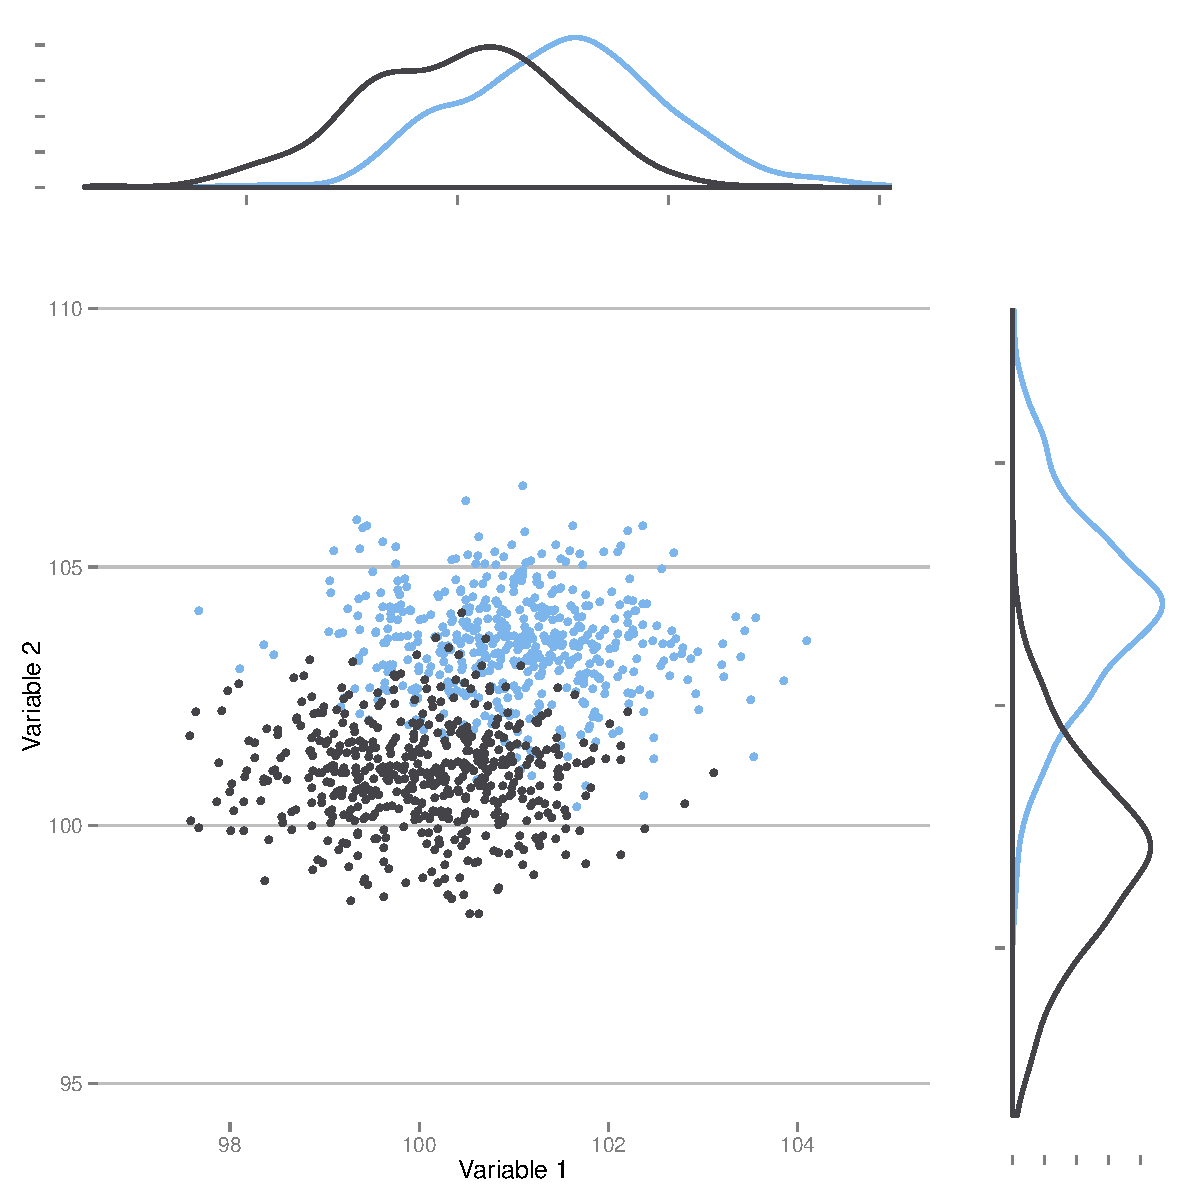
\includegraphics[scale=0.6]{figure/equifinality-variable-effect.pdf}
% \caption{Simple example of the effect of variable choice in distinguishing models.  The variable on the X axis displays quite a bit of overlap between models, while the variable on the Y axis distinguishes the models with fairly high accuracy.}
% \label{img:variables-equifinality-example}
% \end{figure}

\begin{figure}[ht]
\centering
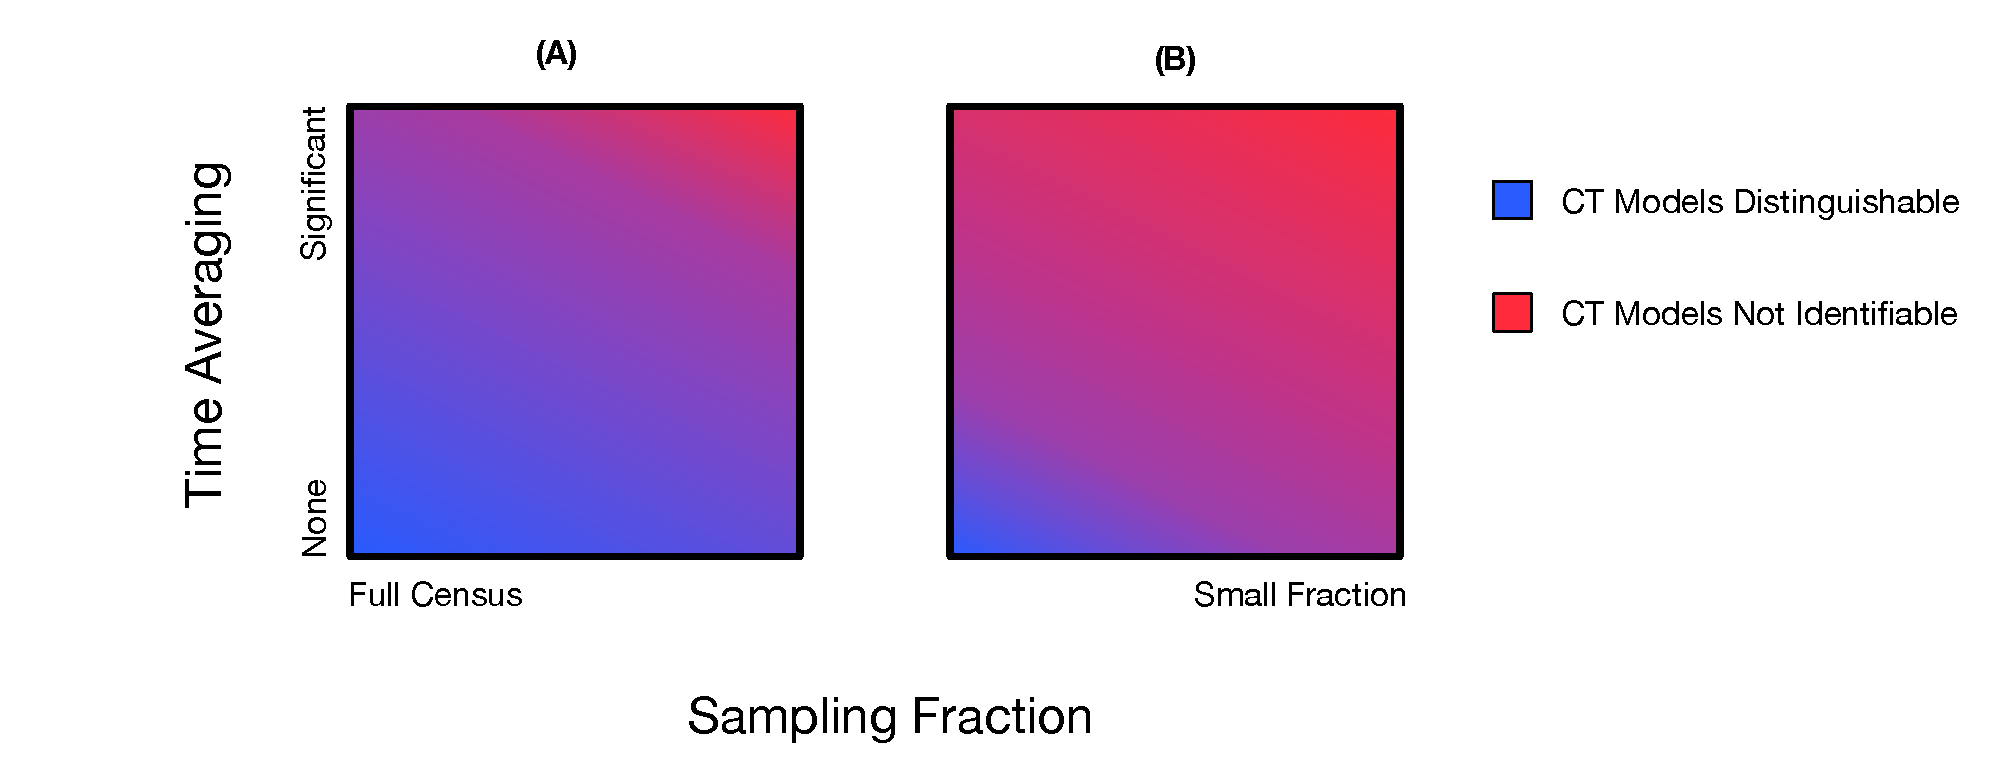
\includegraphics[scale=0.3]{figure/equifinality-transmission-bias-scenarios.pdf}
\caption{foo}
\label{img:fig-1-study-scenarios}
\end{figure}


\begin{figure}[ht]
\centering
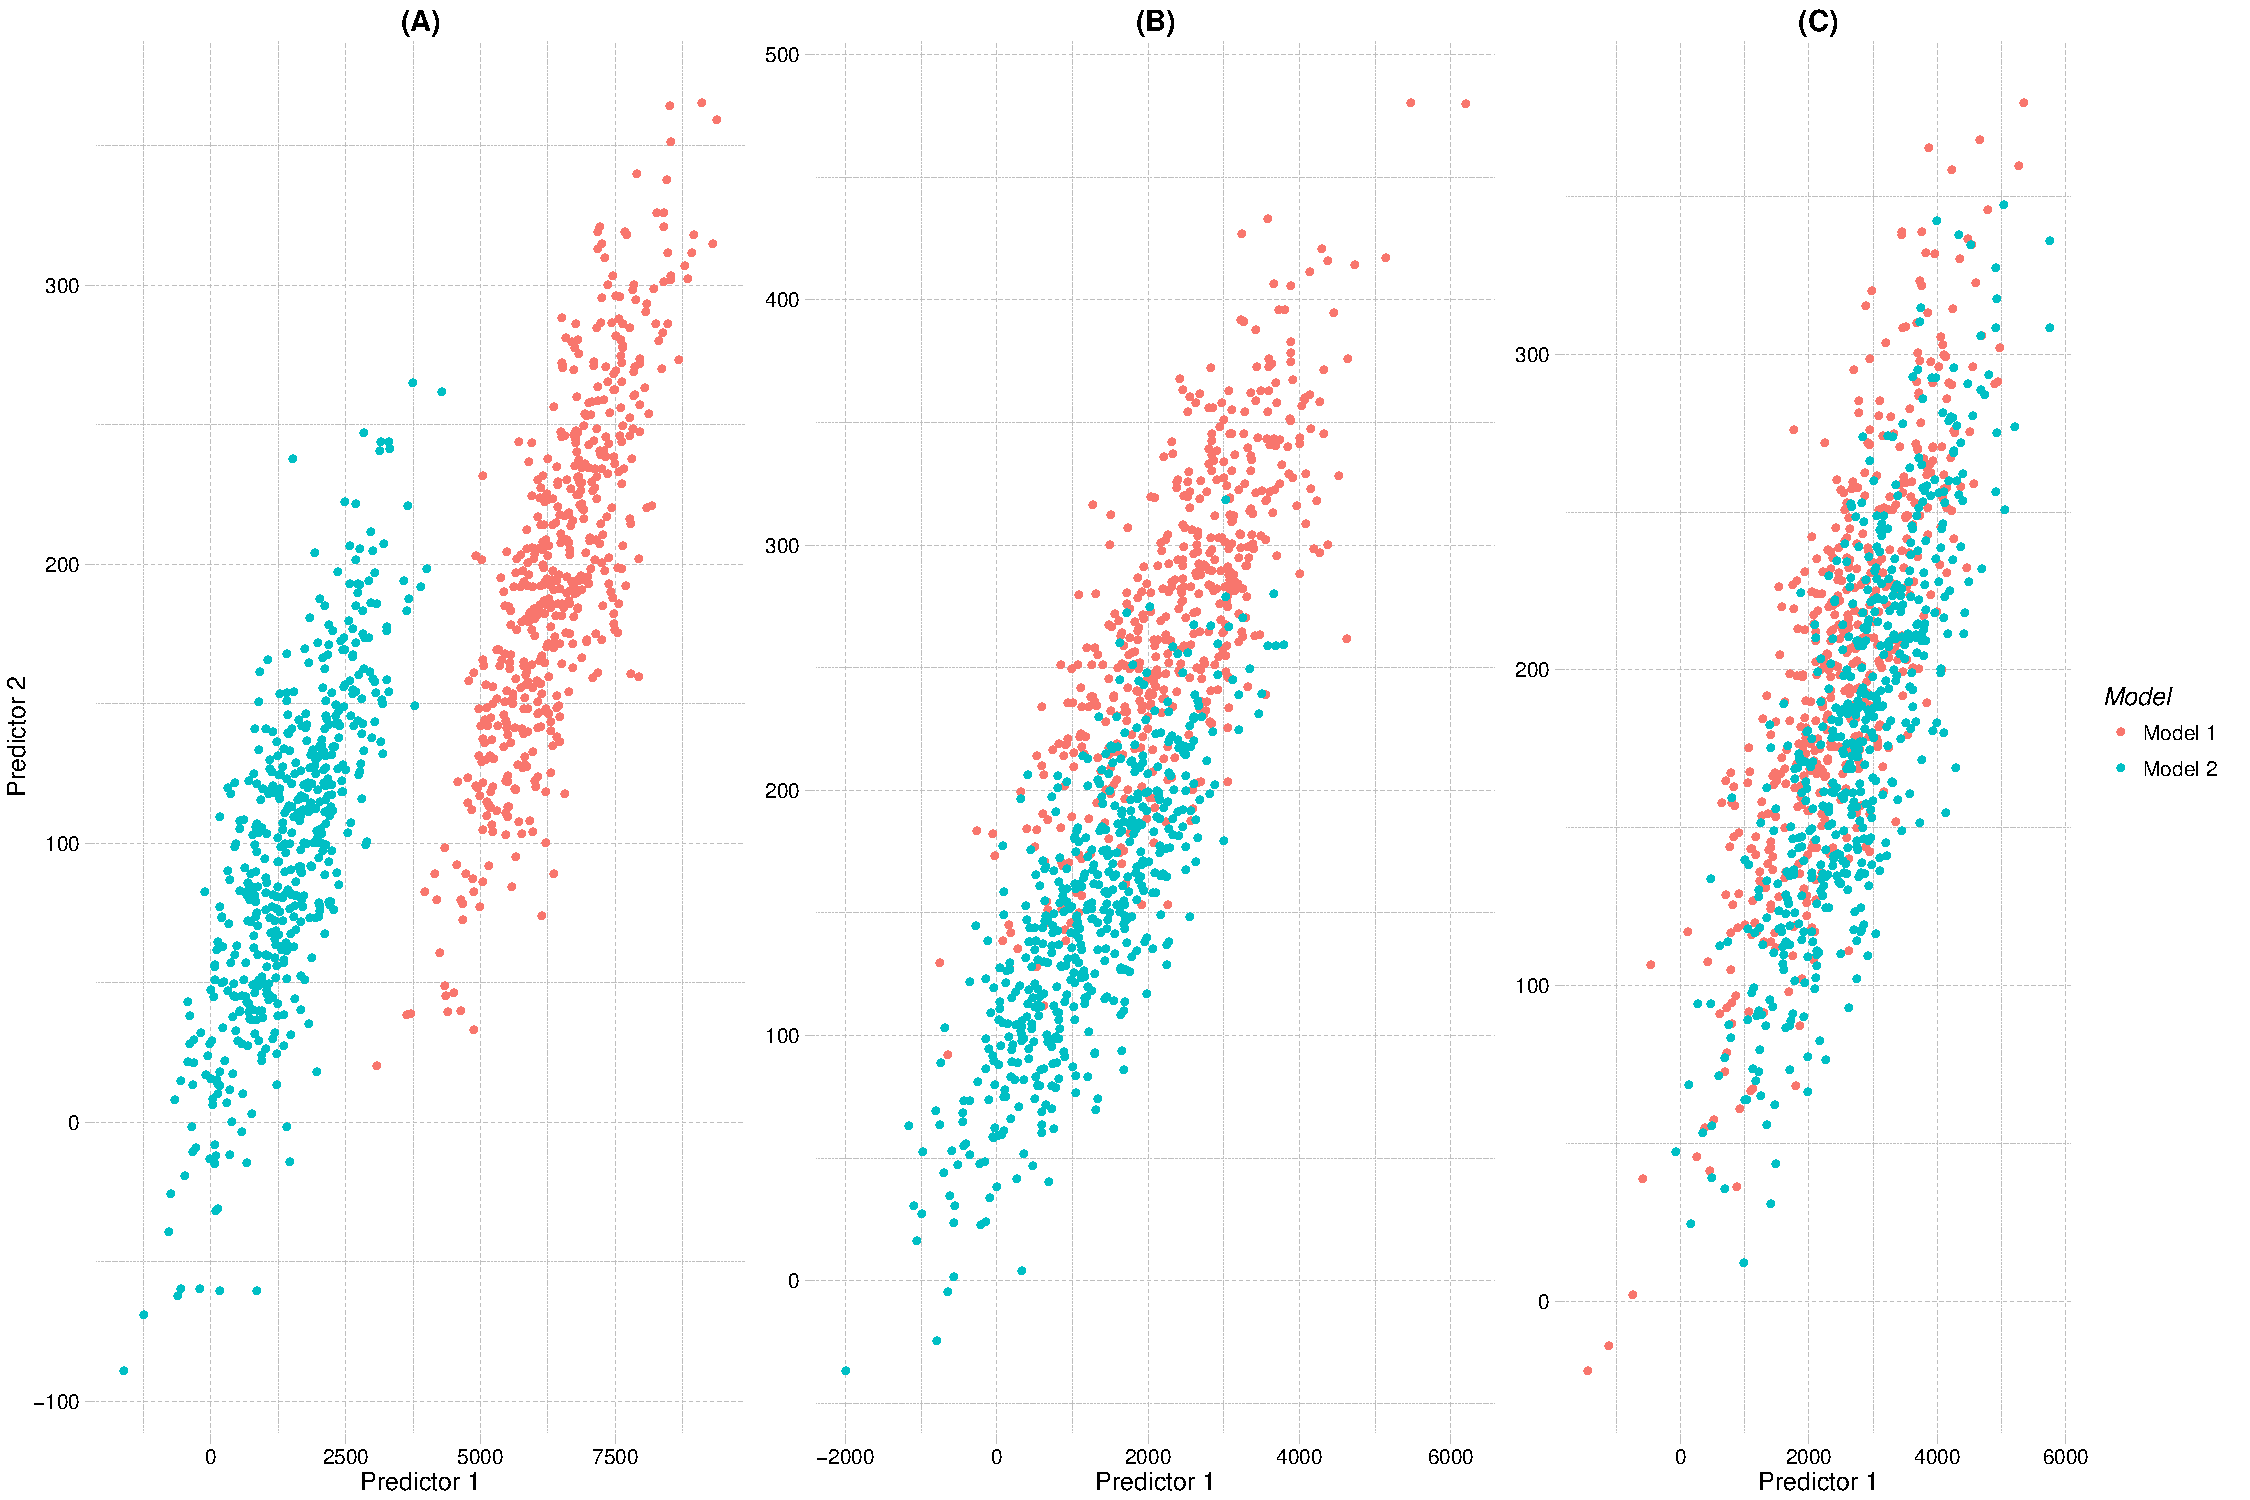
\includegraphics[scale=0.6]{figure/distributional-overlap.pdf}
\caption{Simple example of model outcomes with different degrees of distinguishability: (A) simulated data point from two fully separate models, (B) two models with a limited overlap region, (C) and two models whose outcomes are highly overlapping.}
\label{img:fig-2-separability-example}
\end{figure}

\begin{figure}[ht]
\centering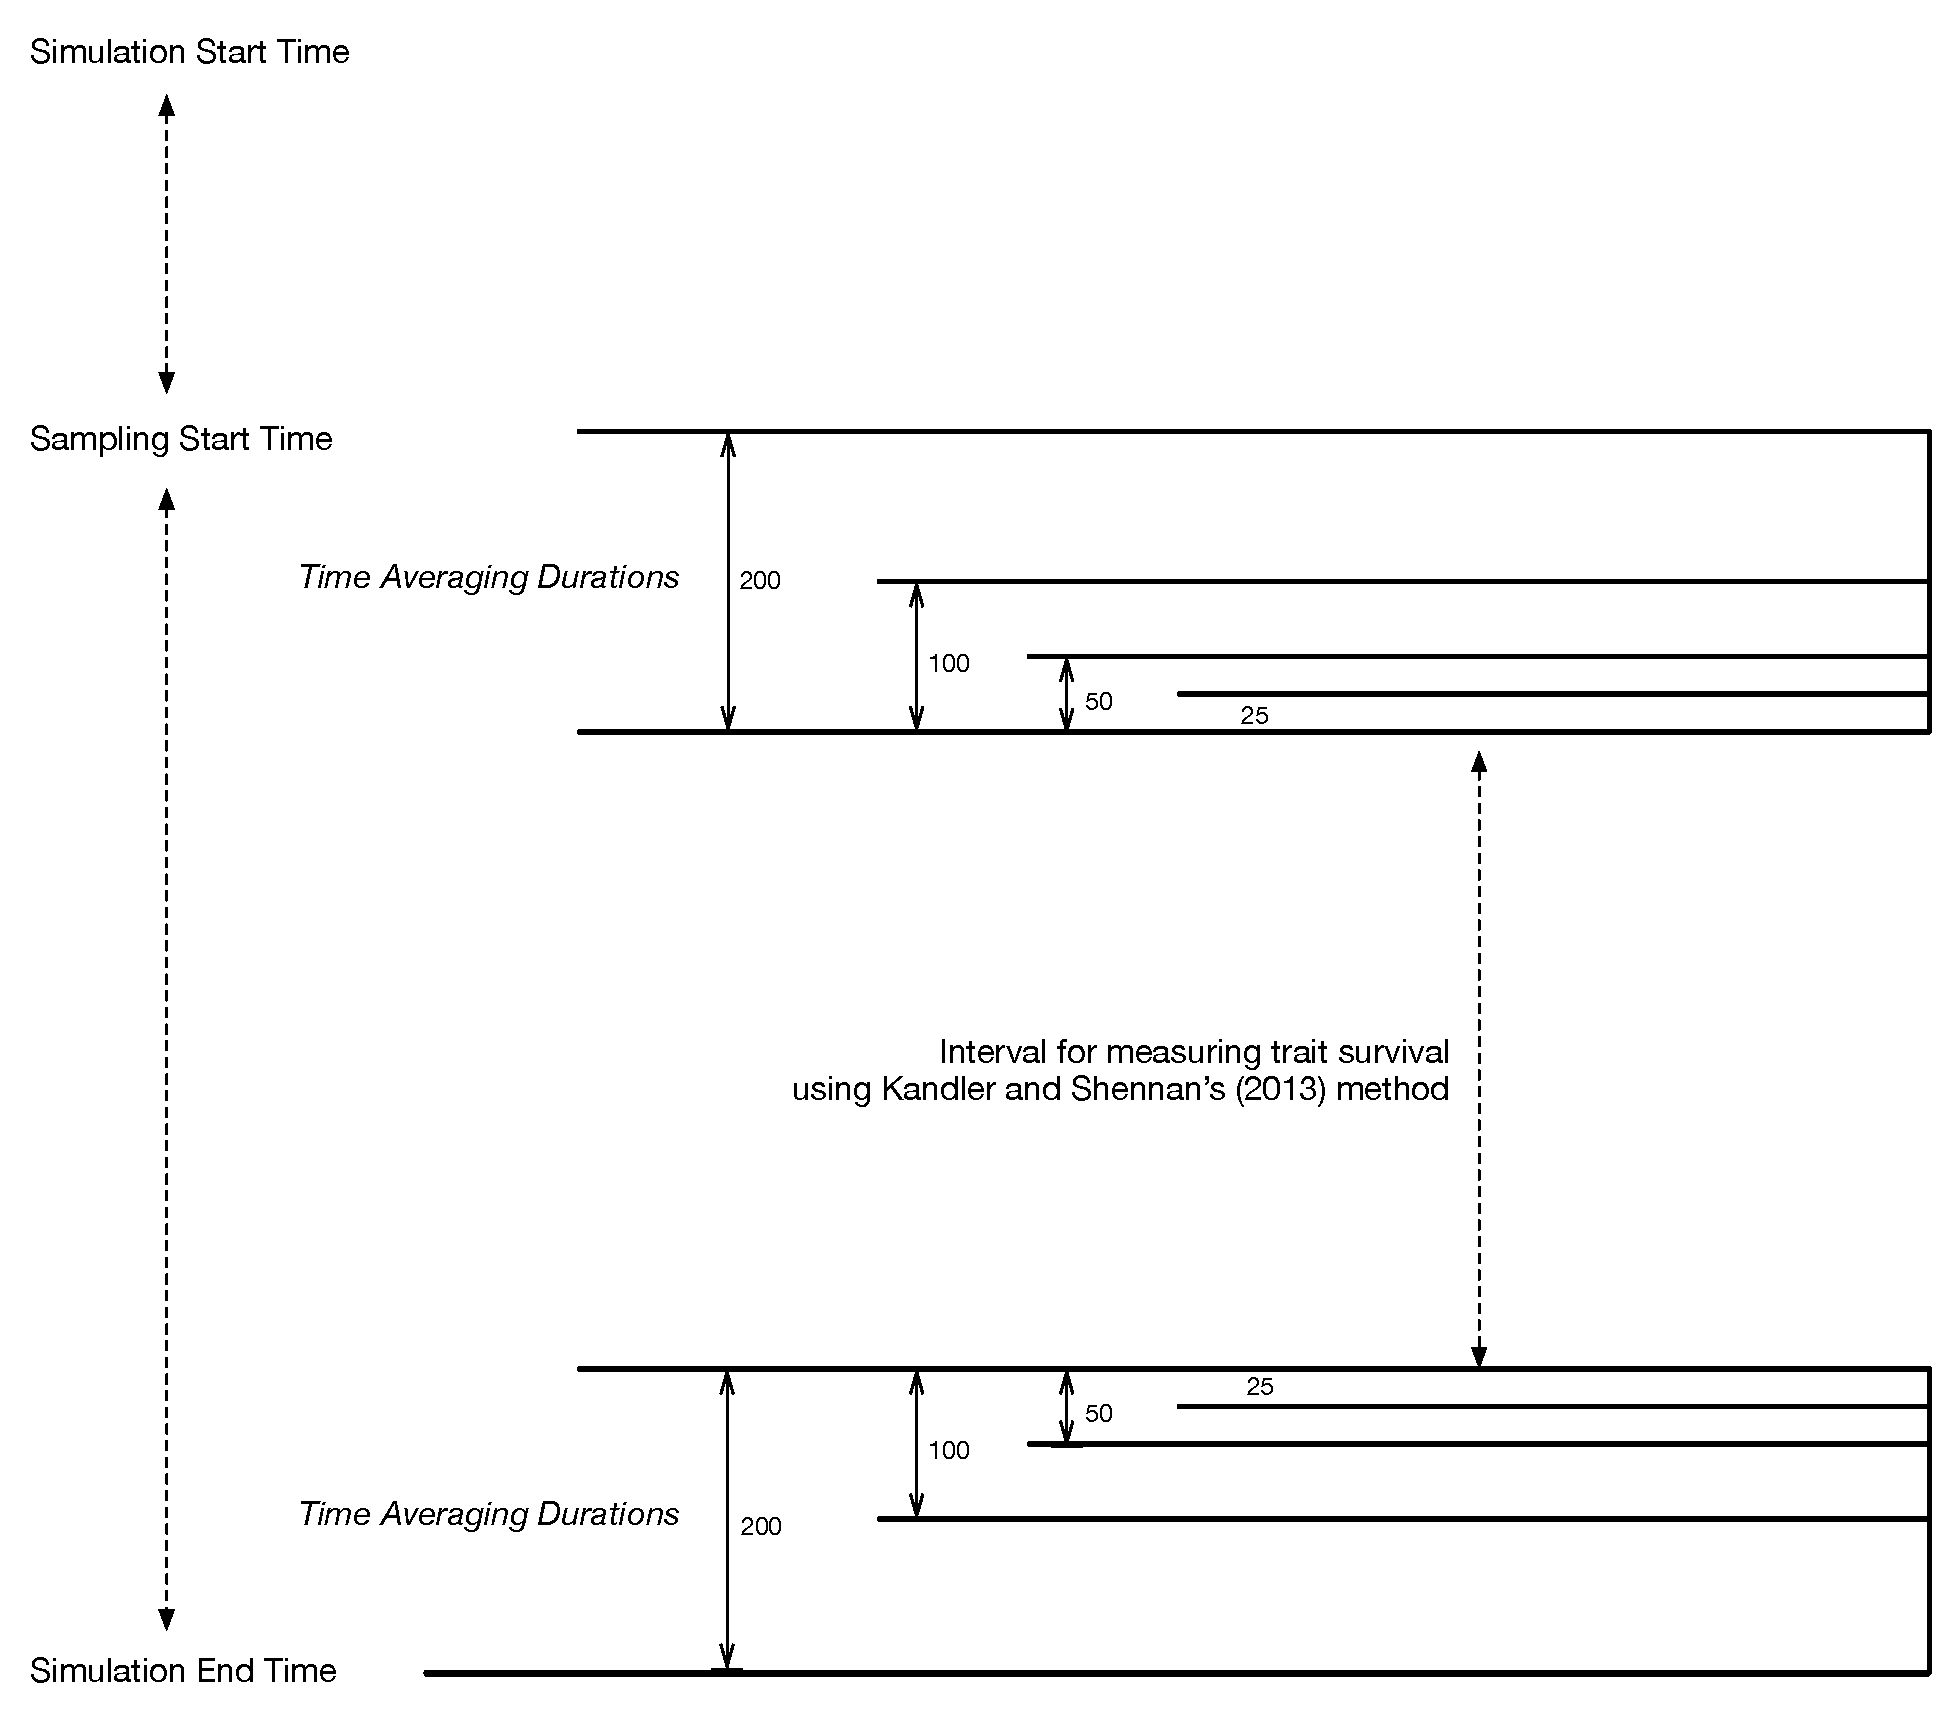
\includegraphics[scale=0.4]{figure/time-averaging-with-kandler-sampling.pdf}
\caption{Schematic of how trait survival as described by Kandler and Shennan \cite{kandler2013non} is extended to time averaged samples of transmission events.  Time runs from the start of the simulation run at the top, to the end at the bottom.  The interval of time over which we calculate the Kandler-Shennan trait survival is given as a simulation parameter, and represents the gap in the middle of the diagram.  Before and after that gap are sampling windows during which transmission events are accumulated over some number of simulated ``generations'' (values of 10, 25, 50, and 100 are used in this paper).  Trait survival is then calculated as the number of traits present in the starting time averaged sample of transmission events, which are still present in the ending time averaged sample of events.}
\label{img:timeaveraging}	
\end{figure}


% \begin{figure}[ht]
% \centering
% 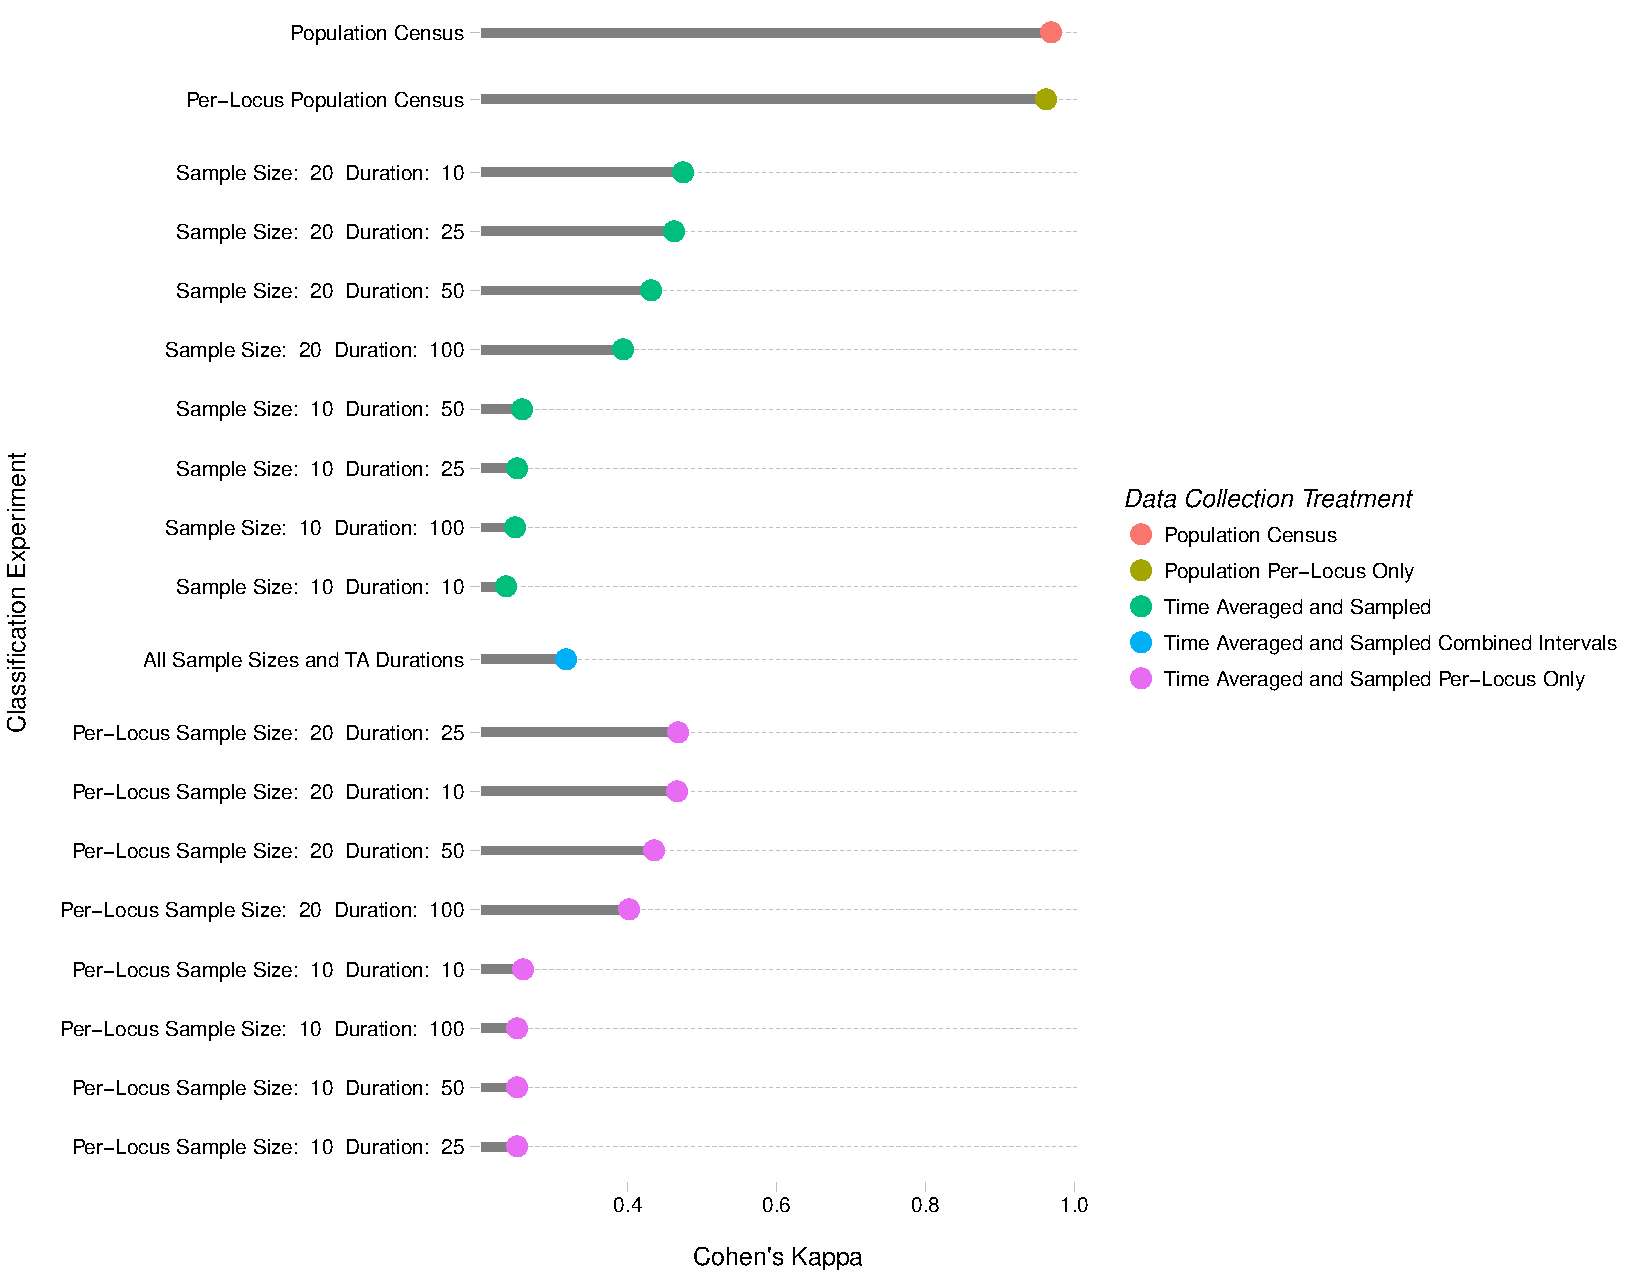
\includegraphics[scale=0.5]{figure/unbiased-biased-kappa-dotchart.pdf}
% \caption{Cohen's kappa for correctly predicting whether simulated data points originate from unbiased copying or any of 3 other biased transmission models.  High values of kappa correspond to high accuracy in correctly distinguishing between transmission models, while values well below 0.5 indicate great difficult and low classifier accuracy.  Each line in the dotchart represents a different data collection treatment, and overall the results indicate that significant equifinality exists except when time averaging is absent and a population census (or near equivalent) is available.}
% \label{img:unbiased-biased-kappa}
% \end{figure}

% \begin{figure}[ht]
% \centering
% 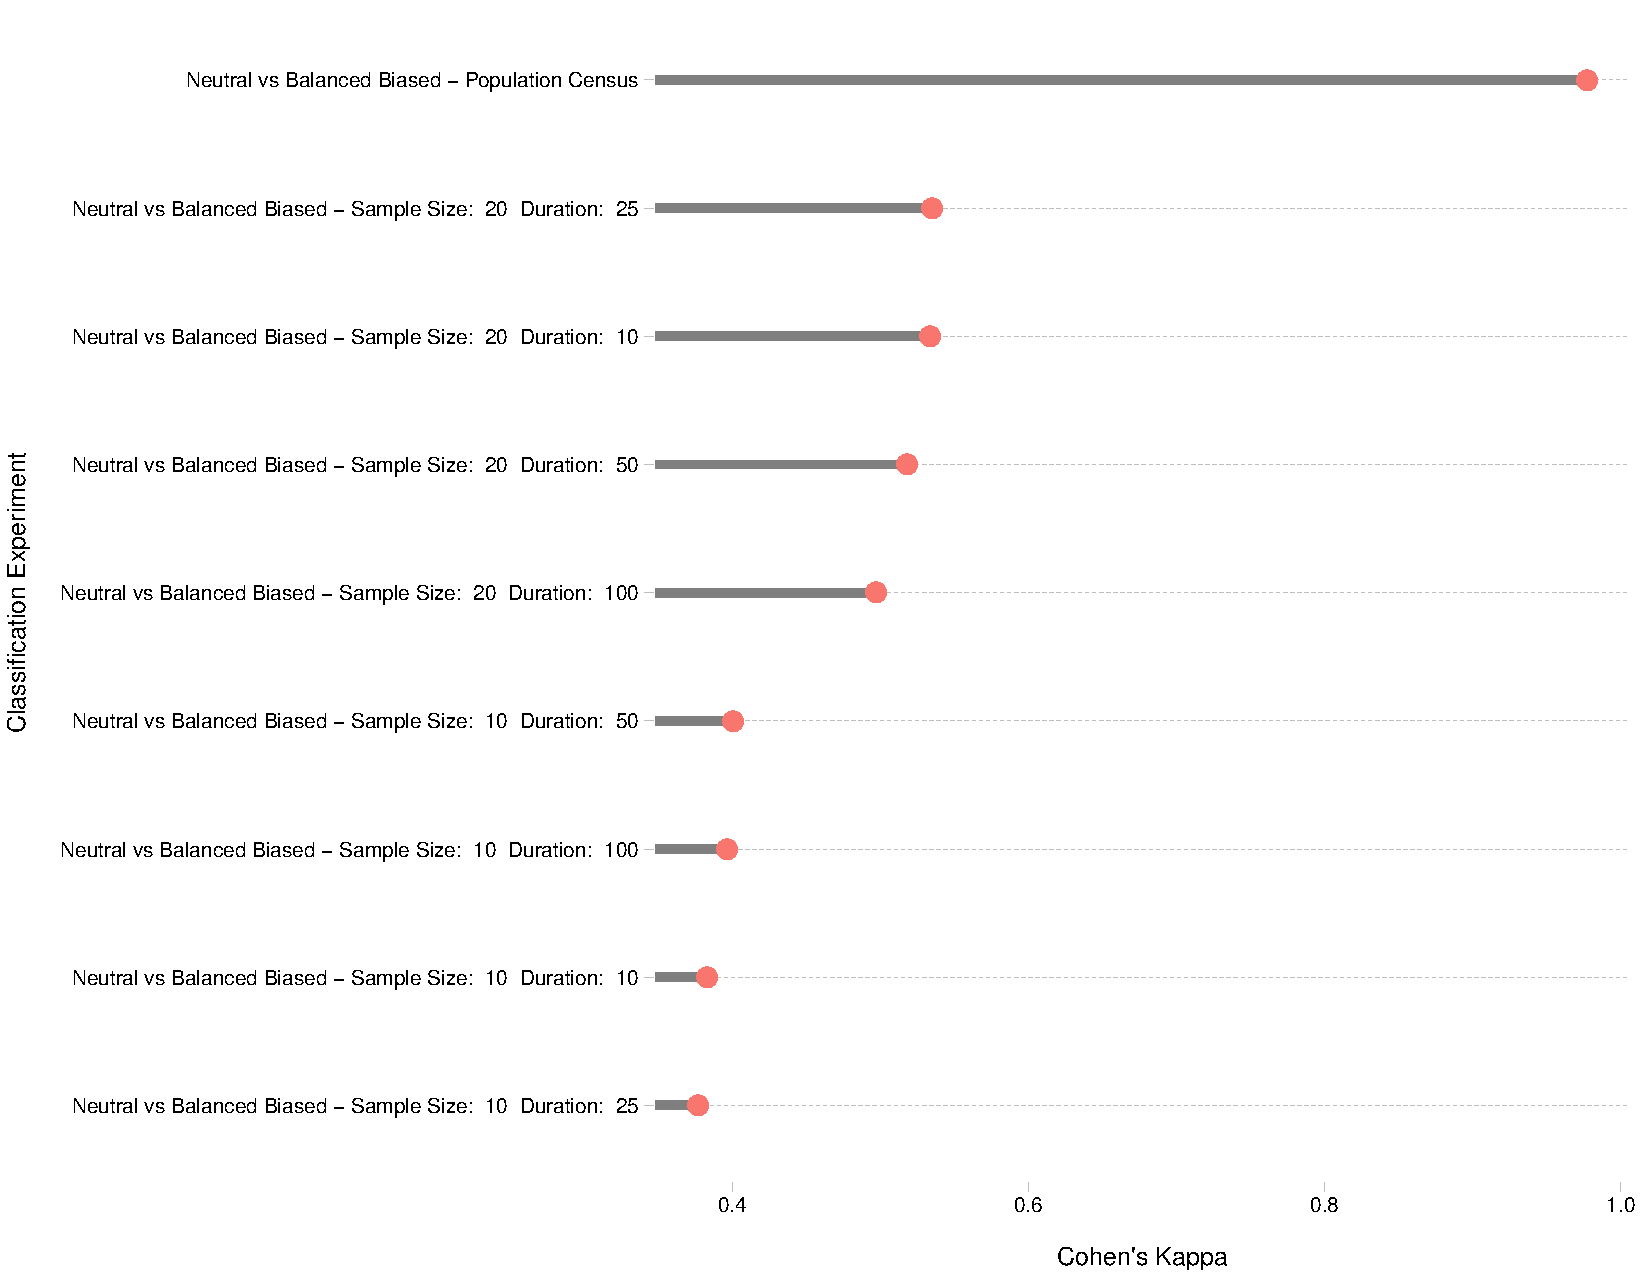
\includegraphics[scale=0.5]{figure/unbiased-balbiased-kappa-dotchart.pdf}
% \caption{Cohen's kappa for correctly predicting whether simulated data points originate from unbiased copying or a balanced mixture of pro- and anti-conformist individuals.  Each line in the dotchart represents a different data collection treatment, and overall the results indicate that significant equifinality exists except when time averaging is absent and a population census (or near equivalent) is available.}
% \label{img:unbiased-biased-kappa}
% \end{figure}

% \begin{figure}[ht]
% \centering
% 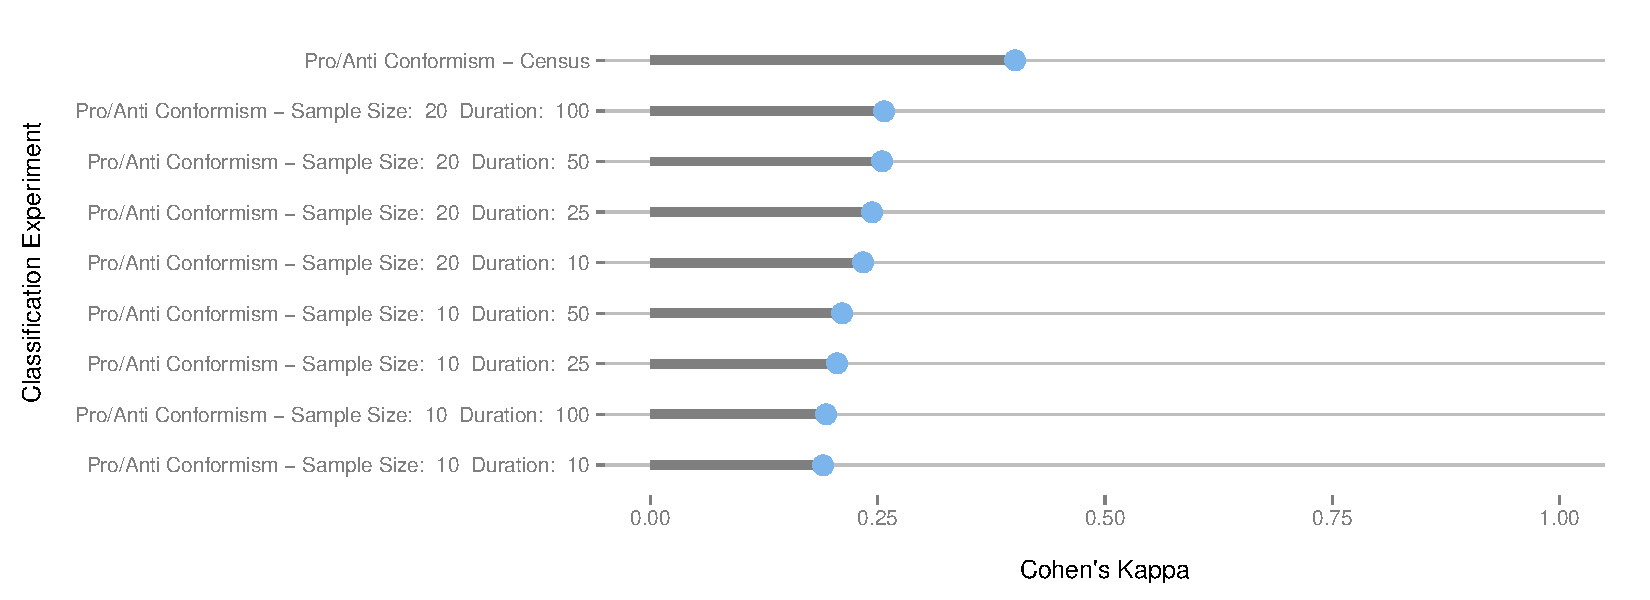
\includegraphics[scale=0.5]{figure/proanticomparison-kappa-dotchart.pdf}
% \caption{Cohen's kappa for correctly predicting whether simulated data points originate from a conformist-dominated mixed population versus a mixed population dominated by anti-conformists.  Each line in the dotchart represents a different data collection treatment, and overall the results indicate that strong equifinality exists regardless of the data collection treatment.}
% \label{img:proanti-kappa}
% \end{figure}

\end{document}

